\chapter{Implémentation du M1}\label{chap:M1}
Dans ce chapitre nous définirons une application \textit{Clients-Serveur} en implémentant le méta-modèle proposé au chapitre \ref{chap:M2}.

\section{Démarche modélisation M1}
L'énoncé du projet/TP nous propose un serveur avec les fonctionnalités suivantes :

\begin{itemize}
\item \verb+ConnexionManager+ : Gestion des connexions. 
\item  \verb+Database+ : Gestion de la base de données.
\item \verb+SecurityManager+ :  Gestion d'un système de sécurité.
\end{itemize}

Un composant étant par définition la spécification d'une fonctionnalité, chacune des fonctionnalités précedement listées est un \verb+Composant+. Chaque service de chaque composant a son port requis relié au rôle requis  du connecteur (et inversement pour les ports et rôles fournis).

Les liaisons entre les différents composants du serveur et le client sont shématisées dans la figure \ref{fig:desSer}. 
\begin{figure}[htb]
  \centering
  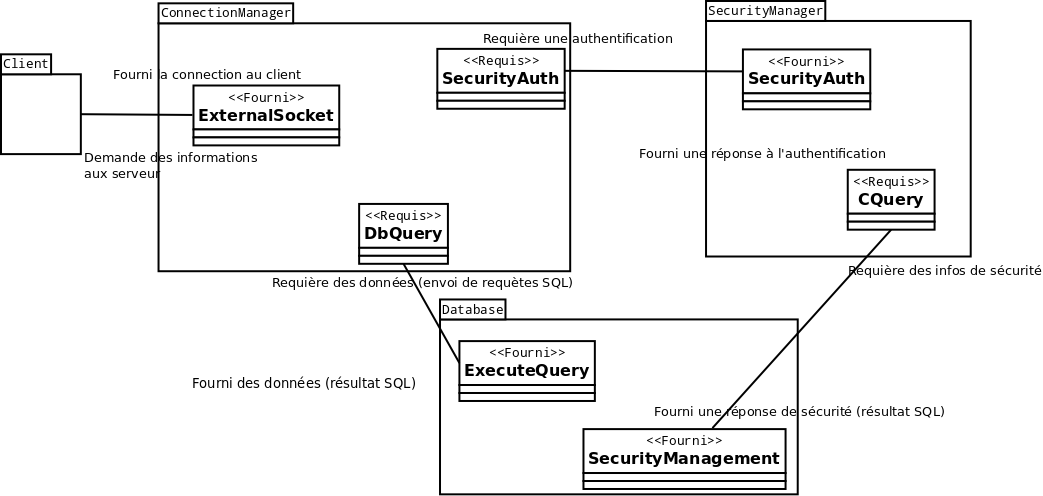
\includegraphics[scale=0.32]{img/DescribServeur}
  \caption{Description du Serveur}
  \label{fig:desSer}.
\end{figure}

Nous retrouvons une version formelle de ce shéma dans la figure \ref{fig:M1} pour la partie \og serveur \fg{} puis dans la figure \ref{fig:M11} pour la partie \og client \fg{} ainsi que sa liaison avec le serveur.


\paragraph{Corrections du M1 après évaluation}
Dans le M1 intialement proposé, on pouvait noter l'absence de \textit{composant serveur}. Pour paller à ce problème nous avons apporté les modifications suivantes : 
\begin{enumerate}
\item Création d'une \verb+ConfigurationServeur+.
\item Mise en place d'un lien \verb+binding+ entre cette configuration et le \verb+Composant+ serveur.
\item Liaison \verb+attachement+ entre les rôles du  \ver+Connecteur+ RPC et le \verb+Composant+ serveur.
\end{enumerate}

Ces modifications sont visibles sur la figure \ref{fig:M11}

\section{Côté Serveur}
\subsection{Déscription des composants serveur}
\subsubsection{ConnexionManager}
Ce composant possède les services suivants : 
\begin{itemize}
\item 
  \verb+ServiceFExternalSocket+ : fournit une connexion au(x) potentiel(s) client(s).
\item 
  \verb+ServicerDDBQuery+ :  requière une réponse de la base de données (requête SQL).
\item 
  \verb+ServiceRSecurityManager+ :  requière une validation de l'authentification.
\end{itemize}

\subsubsection{Database}
Ce composant possède les services suivants : 
\begin{itemize}
\item 
  \verb+ServiceFSecurityManagement+ :  fournit une réponse à la requête de sécurité.
\item 
  \verb+ServicerFExecuteSQL+ :  fournit une réponse à une requête du client (par le ConnexionManager).
\end{itemize}

\subsubsection{SecurityManager}
Ce composant possède les services suivants : 
\begin{itemize}
\item 
  \verb+ServiceFSecurityAuth+ : fournit une validation de la demande de connexion.
\item 
  \verb+ServicerSecurityManager+ :  requière une réponde de sécurité de la base de données (requête SQL).
\end{itemize}

\subsection{Diagramme M1 côté serveur}
\pagestyle{fancy}
\clearpage
\pagestyle{empty}
{
\begin{figure}[htb]
  \centering
  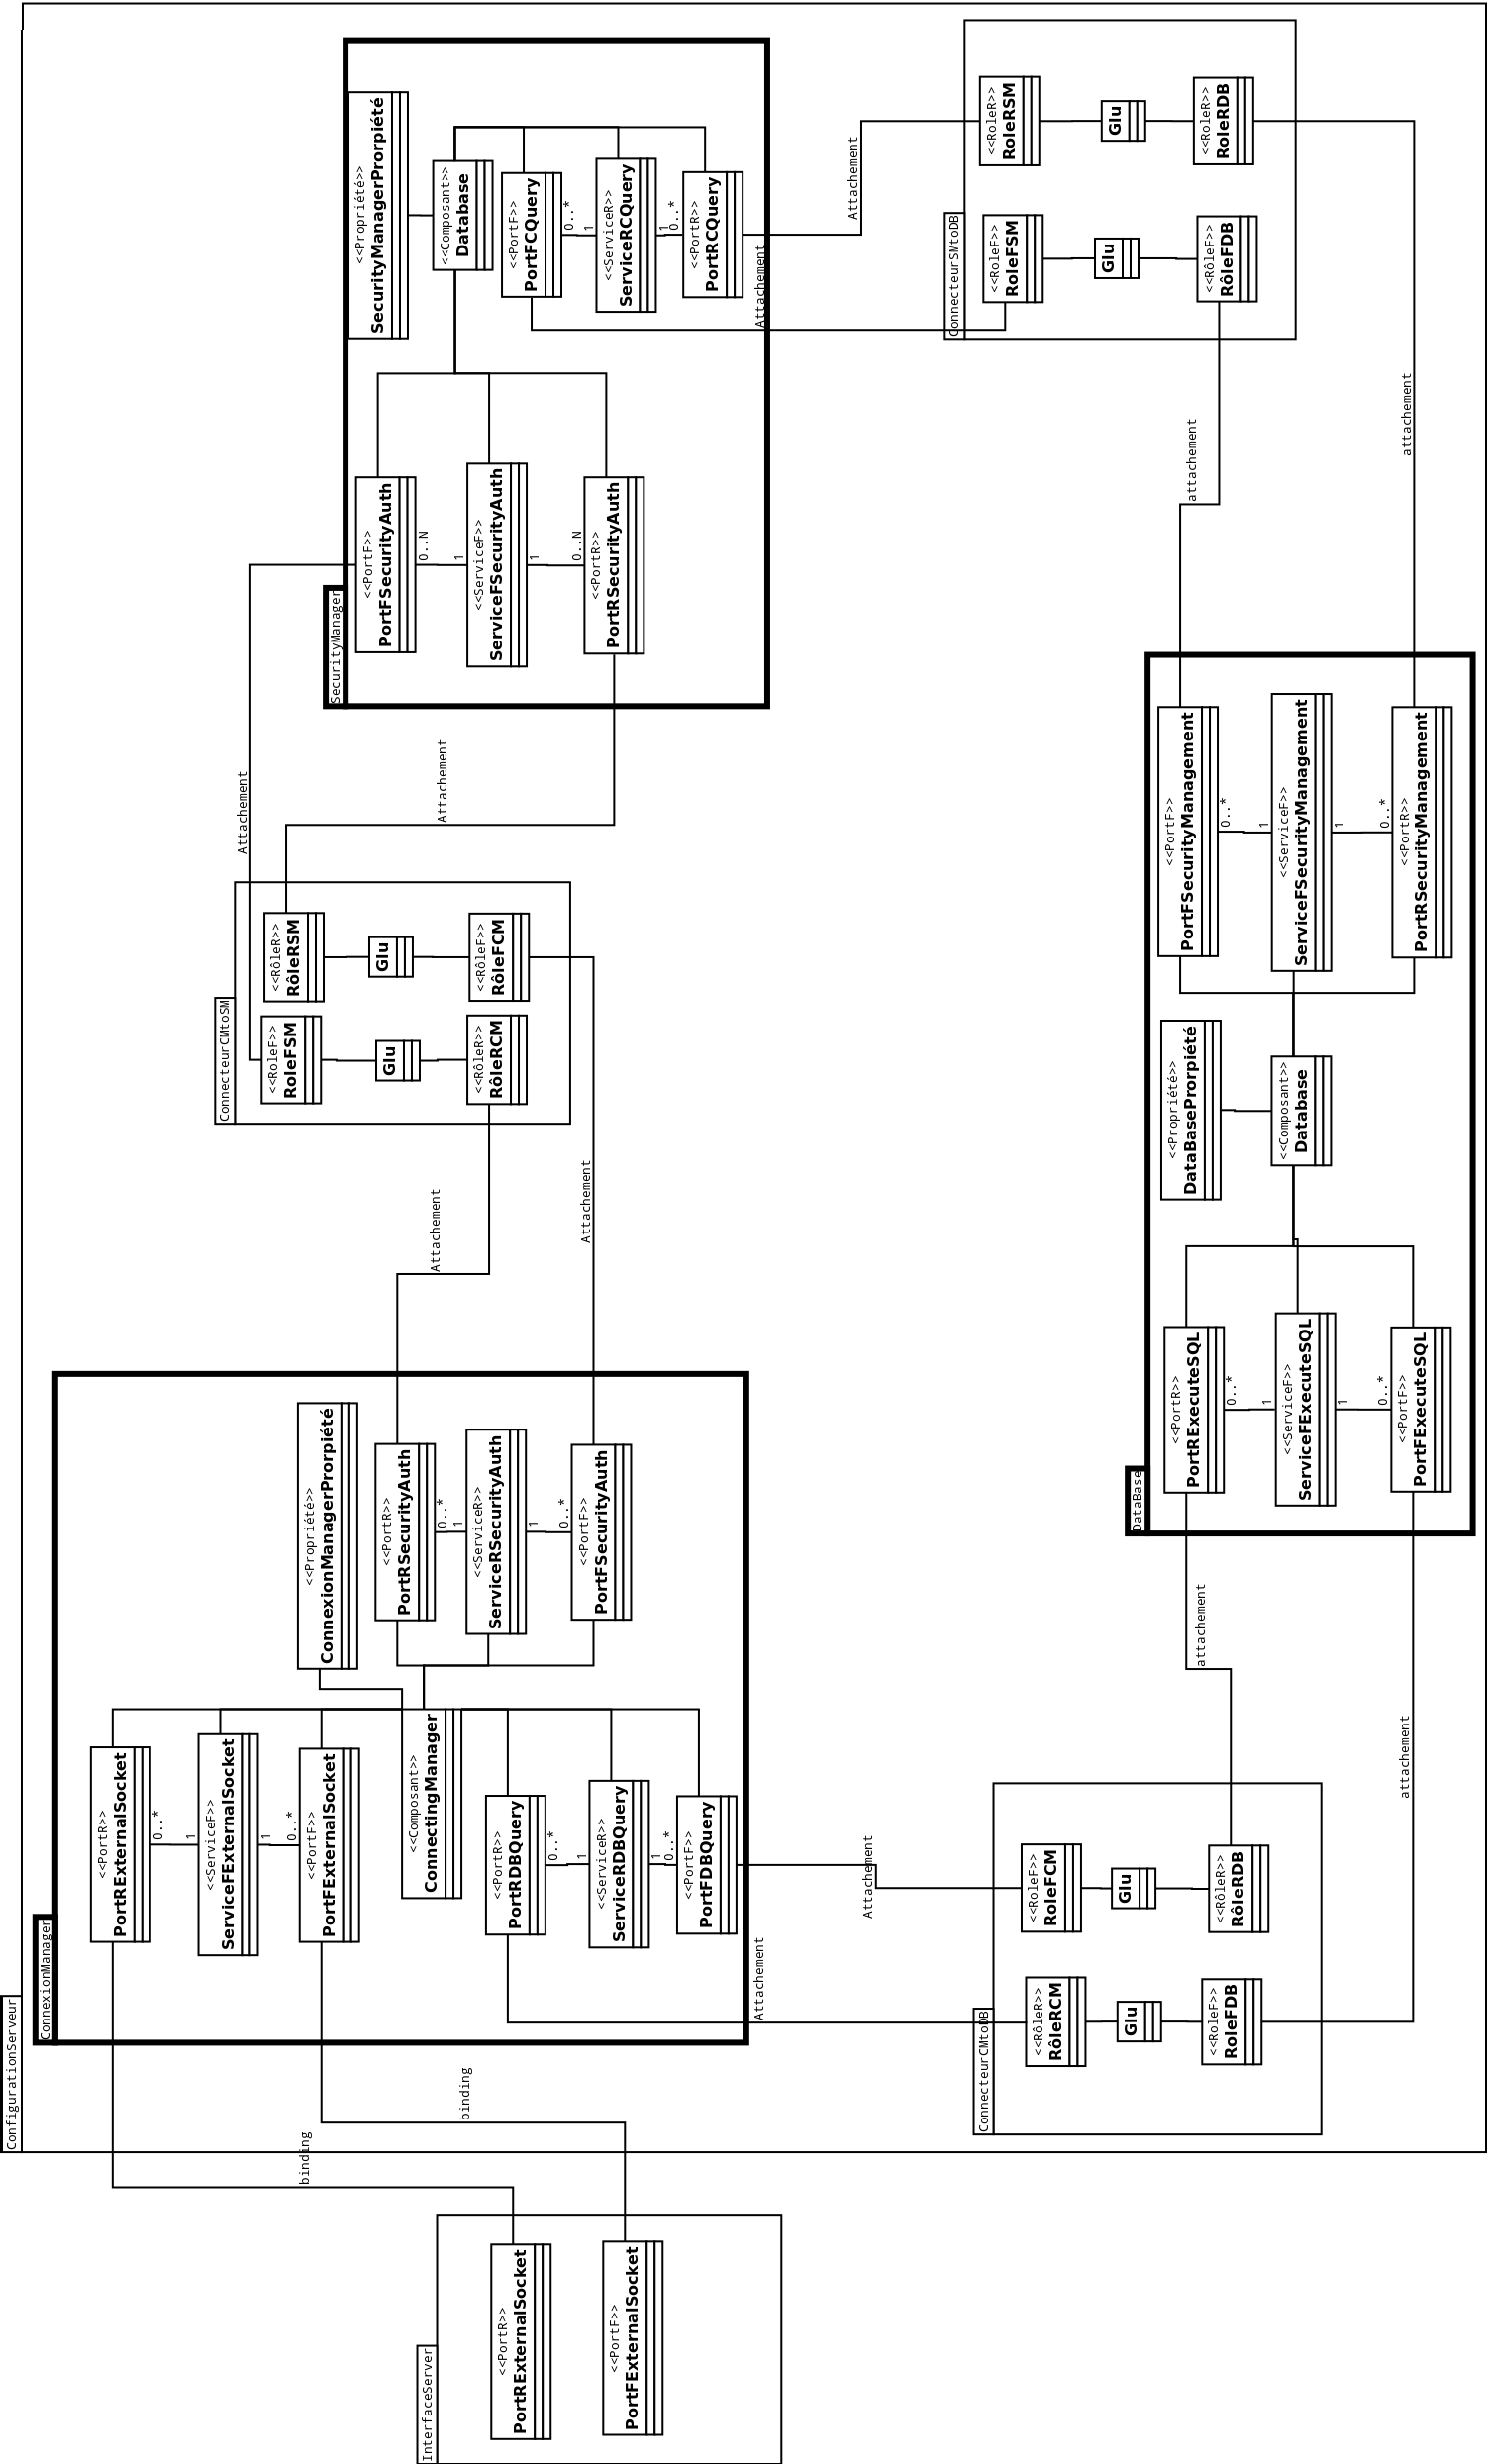
\includegraphics[scale=0.20]{img/M1}
  \caption{Model (M1) côté serveur}
  \label{fig:M1}
\end{figure}
}
\clearpage

\pagestyle{fancy}
\section{Côté Client}
\subsection{Description du Client}
Le client est un composant permettant  à un utilisateur de demander une connexion au serveur à partir d'un login et d'un mot de passe. Une fois connecté, le client peut interroger la base de données du serveur.
 
Le composant client possède le service : 
\begin{itemize}
\item 
  \verb+ServiceRConnexionRPC+ : requière une connexion au serveur.
\end{itemize}
\subsection{Diagramme M1 côté client}
\begin{figure}[htb]
  \centering
  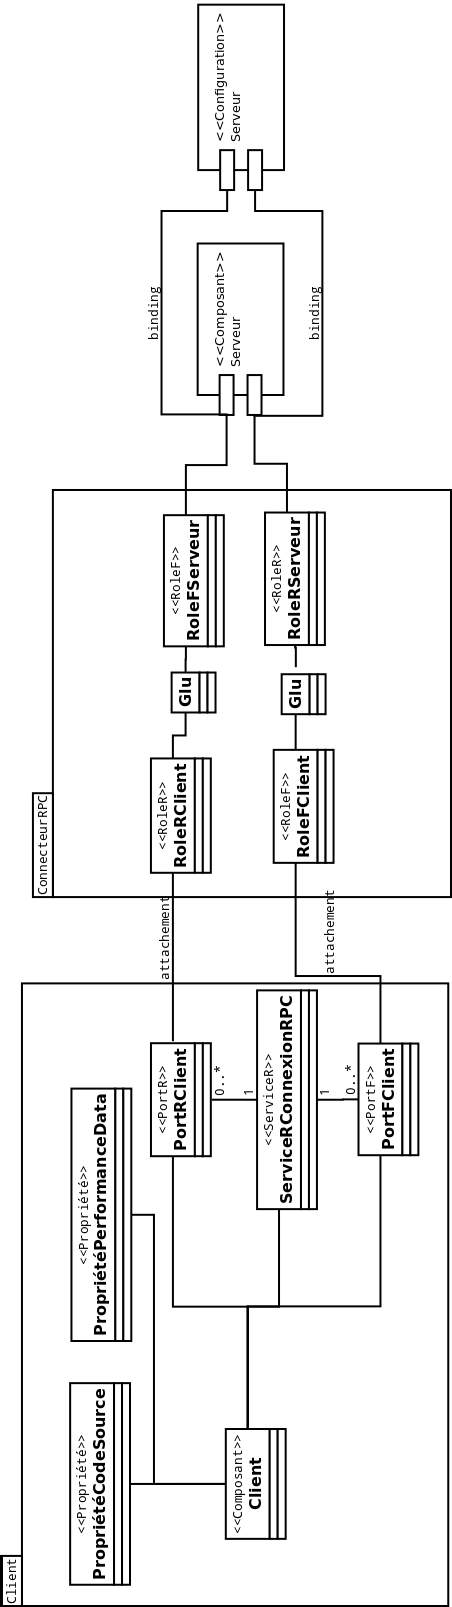
\includegraphics[scale=0.24]{img/M11}
  \caption{Model (M1) côté client}
  \label{fig:M11}
\end{figure}

